\documentclass[twoside]{book}

% Packages required by doxygen
\usepackage{calc}
\usepackage{doxygen}
\usepackage{graphicx}
\usepackage[utf8]{inputenc}
\usepackage{makeidx}
\usepackage{multicol}
\usepackage{multirow}
\PassOptionsToPackage{warn}{textcomp}
\usepackage{textcomp}
\usepackage[nointegrals]{wasysym}
\usepackage[table]{xcolor}

% Font selection
\usepackage[T1]{fontenc}
\usepackage{mathptmx}
\usepackage[scaled=.90]{helvet}
\usepackage{courier}
\usepackage{amssymb}
\usepackage{sectsty}
\renewcommand{\familydefault}{\sfdefault}
\allsectionsfont{%
  \fontseries{bc}\selectfont%
  \color{darkgray}%
}
\renewcommand{\DoxyLabelFont}{%
  \fontseries{bc}\selectfont%
  \color{darkgray}%
}
\newcommand{\+}{\discretionary{\mbox{\scriptsize$\hookleftarrow$}}{}{}}

% Page & text layout
\usepackage{geometry}
\geometry{%
  a4paper,%
  top=2.5cm,%
  bottom=2.5cm,%
  left=2.5cm,%
  right=2.5cm%
}
\tolerance=750
\hfuzz=15pt
\hbadness=750
\setlength{\emergencystretch}{15pt}
\setlength{\parindent}{0cm}
\setlength{\parskip}{0.2cm}
\makeatletter
\renewcommand{\paragraph}{%
  \@startsection{paragraph}{4}{0ex}{-1.0ex}{1.0ex}{%
    \normalfont\normalsize\bfseries\SS@parafont%
  }%
}
\renewcommand{\subparagraph}{%
  \@startsection{subparagraph}{5}{0ex}{-1.0ex}{1.0ex}{%
    \normalfont\normalsize\bfseries\SS@subparafont%
  }%
}
\makeatother

% Headers & footers
\usepackage{fancyhdr}
\pagestyle{fancyplain}
\fancyhead[LE]{\fancyplain{}{\bfseries\thepage}}
\fancyhead[CE]{\fancyplain{}{}}
\fancyhead[RE]{\fancyplain{}{\bfseries\leftmark}}
\fancyhead[LO]{\fancyplain{}{\bfseries\rightmark}}
\fancyhead[CO]{\fancyplain{}{}}
\fancyhead[RO]{\fancyplain{}{\bfseries\thepage}}
\fancyfoot[LE]{\fancyplain{}{}}
\fancyfoot[CE]{\fancyplain{}{}}
\fancyfoot[RE]{\fancyplain{}{\bfseries\scriptsize Generated on Sat Feb 22 2014 22\+:09\+:14 for My Project by Doxygen }}
\fancyfoot[LO]{\fancyplain{}{\bfseries\scriptsize Generated on Sat Feb 22 2014 22\+:09\+:14 for My Project by Doxygen }}
\fancyfoot[CO]{\fancyplain{}{}}
\fancyfoot[RO]{\fancyplain{}{}}
\renewcommand{\footrulewidth}{0.4pt}
\renewcommand{\chaptermark}[1]{%
  \markboth{#1}{}%
}
\renewcommand{\sectionmark}[1]{%
  \markright{\thesection\ #1}%
}

% Indices & bibliography
\usepackage{natbib}
\usepackage[titles]{tocloft}
\setcounter{tocdepth}{3}
\setcounter{secnumdepth}{5}
\makeindex

% Hyperlinks (required, but should be loaded last)
\usepackage{ifpdf}
\ifpdf
  \usepackage[pdftex,pagebackref=true]{hyperref}
\else
  \usepackage[ps2pdf,pagebackref=true]{hyperref}
\fi
\hypersetup{%
  colorlinks=true,%
  linkcolor=blue,%
  citecolor=blue,%
  unicode%
}

% Custom commands
\newcommand{\clearemptydoublepage}{%
  \newpage{\pagestyle{empty}\cleardoublepage}%
}


%===== C O N T E N T S =====

\begin{document}

% Titlepage & ToC
\hypersetup{pageanchor=false,
             bookmarks=true,
             bookmarksnumbered=true,
             pdfencoding=unicode
            }
\pagenumbering{roman}
\begin{titlepage}
\vspace*{7cm}
\begin{center}%
{\Large My Project }\\
\vspace*{1cm}
{\large Generated by Doxygen 1.8.6}\\
\vspace*{0.5cm}
{\small Sat Feb 22 2014 22:09:14}\\
\end{center}
\end{titlepage}
\clearemptydoublepage
\tableofcontents
\clearemptydoublepage
\pagenumbering{arabic}
\hypersetup{pageanchor=true}

%--- Begin generated contents ---
\chapter{Hierarchical Index}
\section{Class Hierarchy}
This inheritance list is sorted roughly, but not completely, alphabetically\+:\begin{DoxyCompactList}
\item Q\+G\+L\+Widget\begin{DoxyCompactList}
\item \contentsline{section}{glrenderer}{\pageref{classglrenderer}}{}
\end{DoxyCompactList}
\item Q\+Main\+Window\begin{DoxyCompactList}
\item \contentsline{section}{Main\+Window}{\pageref{class_main_window}}{}
\end{DoxyCompactList}
\item Sound\+Stream\begin{DoxyCompactList}
\item \contentsline{section}{sfe\+:\+:Sequential\+Sound\+Streamer}{\pageref{classsfe_1_1_sequential_sound_streamer}}{}
\end{DoxyCompactList}
\item \contentsline{section}{Turing}{\pageref{class_turing}}{}
\item \contentsline{section}{Ui\+\_\+\+Main\+Window}{\pageref{class_ui___main_window}}{}
\begin{DoxyCompactList}
\item \contentsline{section}{Ui\+:\+:Main\+Window}{\pageref{class_ui_1_1_main_window}}{}
\end{DoxyCompactList}
\end{DoxyCompactList}

\chapter{Class Index}
\section{Class List}
Here are the classes, structs, unions and interfaces with brief descriptions\+:\begin{DoxyCompactList}
\item\contentsline{section}{\hyperlink{classglrenderer}{glrenderer} }{\pageref{classglrenderer}}{}
\item\contentsline{section}{\hyperlink{class_main_window}{Main\+Window} }{\pageref{class_main_window}}{}
\item\contentsline{section}{\hyperlink{class_ui_1_1_main_window}{Ui\+::\+Main\+Window} }{\pageref{class_ui_1_1_main_window}}{}
\item\contentsline{section}{\hyperlink{classsfe_1_1_sequential_sound_streamer}{sfe\+::\+Sequential\+Sound\+Streamer} }{\pageref{classsfe_1_1_sequential_sound_streamer}}{}
\item\contentsline{section}{\hyperlink{class_turing}{Turing} }{\pageref{class_turing}}{}
\item\contentsline{section}{\hyperlink{class_ui___main_window}{Ui\+\_\+\+Main\+Window} }{\pageref{class_ui___main_window}}{}
\end{DoxyCompactList}

\chapter{Class Documentation}
\hypertarget{classsfe_1_1_sequential_sound_streamer}{\section{sfe\+:\+:Sequential\+Sound\+Streamer Class Reference}
\label{classsfe_1_1_sequential_sound_streamer}\index{sfe\+::\+Sequential\+Sound\+Streamer@{sfe\+::\+Sequential\+Sound\+Streamer}}
}
Inheritance diagram for sfe\+:\+:Sequential\+Sound\+Streamer\+:\begin{figure}[H]
\begin{center}
\leavevmode
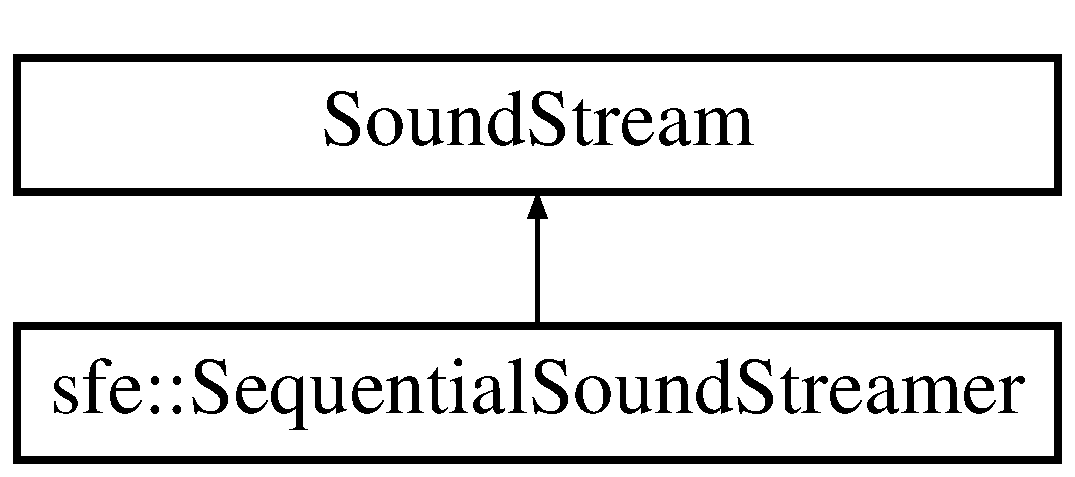
\includegraphics[height=2.000000cm]{classsfe_1_1_sequential_sound_streamer}
\end{center}
\end{figure}
\subsection*{Public Member Functions}
\begin{DoxyCompactItemize}
\item 
\hypertarget{classsfe_1_1_sequential_sound_streamer_a0889a532e125e6229911c87a4411149b}{{\bfseries Sequential\+Sound\+Streamer} (std\+::size\+\_\+t Buffer\+Size)}\label{classsfe_1_1_sequential_sound_streamer_a0889a532e125e6229911c87a4411149b}

\item 
void \hyperlink{classsfe_1_1_sequential_sound_streamer_a650824533bf27a504739798fc4291e69}{load} (const sf\+::\+Sound\+Buffer \&buffer)
\item 
double $\ast$ \hyperlink{classsfe_1_1_sequential_sound_streamer_a54215b061173c1c6b1bebe73a8e79cf0}{get\+F\+F\+T\+Abs} ()
\item 
double $\ast$ \hyperlink{classsfe_1_1_sequential_sound_streamer_a7c94675b37f7f18ae3b535b1c358fb3b}{get\+F\+F\+T\+Phase} ()
\end{DoxyCompactItemize}


\subsection{Member Function Documentation}
\hypertarget{classsfe_1_1_sequential_sound_streamer_a54215b061173c1c6b1bebe73a8e79cf0}{\index{sfe\+::\+Sequential\+Sound\+Streamer@{sfe\+::\+Sequential\+Sound\+Streamer}!get\+F\+F\+T\+Abs@{get\+F\+F\+T\+Abs}}
\index{get\+F\+F\+T\+Abs@{get\+F\+F\+T\+Abs}!sfe\+::\+Sequential\+Sound\+Streamer@{sfe\+::\+Sequential\+Sound\+Streamer}}
\subsubsection[{get\+F\+F\+T\+Abs}]{\setlength{\rightskip}{0pt plus 5cm}double$\ast$ sfe\+::\+Sequential\+Sound\+Streamer\+::get\+F\+F\+T\+Abs (
\begin{DoxyParamCaption}
{}
\end{DoxyParamCaption}
)\hspace{0.3cm}{\ttfamily [inline]}}}\label{classsfe_1_1_sequential_sound_streamer_a54215b061173c1c6b1bebe73a8e79cf0}
returns an array of the magnitude of the transformed data \hypertarget{classsfe_1_1_sequential_sound_streamer_a7c94675b37f7f18ae3b535b1c358fb3b}{\index{sfe\+::\+Sequential\+Sound\+Streamer@{sfe\+::\+Sequential\+Sound\+Streamer}!get\+F\+F\+T\+Phase@{get\+F\+F\+T\+Phase}}
\index{get\+F\+F\+T\+Phase@{get\+F\+F\+T\+Phase}!sfe\+::\+Sequential\+Sound\+Streamer@{sfe\+::\+Sequential\+Sound\+Streamer}}
\subsubsection[{get\+F\+F\+T\+Phase}]{\setlength{\rightskip}{0pt plus 5cm}double$\ast$ sfe\+::\+Sequential\+Sound\+Streamer\+::get\+F\+F\+T\+Phase (
\begin{DoxyParamCaption}
{}
\end{DoxyParamCaption}
)\hspace{0.3cm}{\ttfamily [inline]}}}\label{classsfe_1_1_sequential_sound_streamer_a7c94675b37f7f18ae3b535b1c358fb3b}
returns an array of the phase of the transformed data \hypertarget{classsfe_1_1_sequential_sound_streamer_a650824533bf27a504739798fc4291e69}{\index{sfe\+::\+Sequential\+Sound\+Streamer@{sfe\+::\+Sequential\+Sound\+Streamer}!load@{load}}
\index{load@{load}!sfe\+::\+Sequential\+Sound\+Streamer@{sfe\+::\+Sequential\+Sound\+Streamer}}
\subsubsection[{load}]{\setlength{\rightskip}{0pt plus 5cm}void sfe\+::\+Sequential\+Sound\+Streamer\+::load (
\begin{DoxyParamCaption}
\item[{const sf\+::\+Sound\+Buffer \&}]{buffer}
\end{DoxyParamCaption}
)}}\label{classsfe_1_1_sequential_sound_streamer_a650824533bf27a504739798fc4291e69}
loads data from a sound buffer object 

The documentation for this class was generated from the following files\+:\begin{DoxyCompactItemize}
\item 
Sequential\+Sound\+Streamer.\+h\item 
Sequential\+Sound\+Streamer.\+cpp\end{DoxyCompactItemize}

%--- End generated contents ---

% Index
\newpage
\phantomsection
\addcontentsline{toc}{chapter}{Index}
\printindex

\end{document}
